\section{Financial\_\-Note  Class Reference}
\label{classFinancial__Note}\index{Financial_Note@{Financial\_\-Note}}
{\tt \#include $<$dil2al.hh$>$}

Inheritance diagram for Financial\_\-Note::\begin{figure}[H]
\begin{center}
\leavevmode
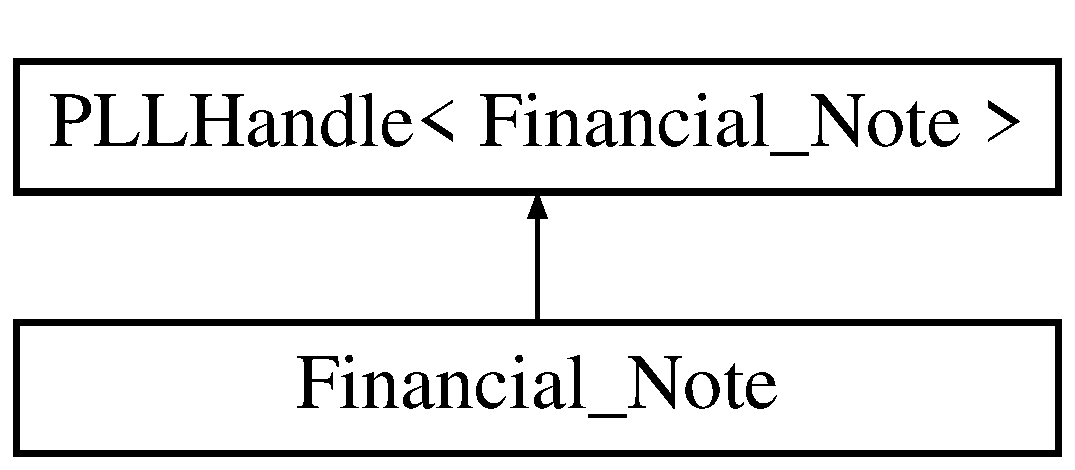
\includegraphics[height=2cm]{classFinancial__Note}
\end{center}
\end{figure}
\subsection*{Public Methods}
\begin{CompactItemize}
\item 
{\bf Financial\_\-Note} (time\_\-t d, double e, {\bf String} t, bool h, {\bf String} n, {\bf String} c)
\item 
{\bf Financial\_\-Note} ()
\item 
{\bf Financial\_\-Note} ({\bf String} \&s, time\_\-t \&t, int \&sloc)
\item 
int {\bf get} ({\bf String} \&s, time\_\-t \&t, int sloc=0)
\item 
{\bf String} {\bf put} () const
\item 
void {\bf link\_\-sorted} ({\bf PLLRoot}$<$ Financial\_\-Note $>$ \&r)
\item 
time\_\-t {\bf Date} () const
\item 
bool {\bf Handled} () const
\item 
{\bf String} {\bf Type} () const
\item 
double {\bf Expense} () const
\end{CompactItemize}
\subsection*{Protected Attributes}
\begin{CompactItemize}
\item 
time\_\-t {\bf date}
\item 
double {\bf expense}
\item 
{\bf String} {\bf type}
\item 
bool {\bf handled}
\item 
{\bf String} {\bf note}
\item 
{\bf String} {\bf comment}
\end{CompactItemize}


\subsection{Constructor \& Destructor Documentation}
\index{Financial_Note@{Financial\_\-Note}!Financial_Note@{Financial\_\-Note}}
\index{Financial_Note@{Financial\_\-Note}!Financial_Note@{Financial\_\-Note}}
\subsubsection{\setlength{\rightskip}{0pt plus 5cm}Financial\_\-Note::Financial\_\-Note (time\_\-t {\em d}, double {\em e}, {\bf String} {\em t}, bool {\em h}, {\bf String} {\em n}, {\bf String} {\em c})\hspace{0.3cm}{\tt  [inline]}}\label{classFinancial__Note_a0}




Definition at line 1083 of file dil2al.hh.

References date, expense, and handled.



\footnotesize\begin{verbatim}1083 : date(d), expense(e), type(t), handled(h), note(n), comment(c) {}
\end{verbatim}\normalsize 
\index{Financial_Note@{Financial\_\-Note}!Financial_Note@{Financial\_\-Note}}
\index{Financial_Note@{Financial\_\-Note}!Financial_Note@{Financial\_\-Note}}
\subsubsection{\setlength{\rightskip}{0pt plus 5cm}Financial\_\-Note::Financial\_\-Note ()\hspace{0.3cm}{\tt  [inline]}}\label{classFinancial__Note_a1}




Definition at line 1084 of file dil2al.hh.

References date, expense, false, and handled.



\footnotesize\begin{verbatim}1084 : date(0), expense(0.0), type(""), handled(false), note(""), comment("") {}
\end{verbatim}\normalsize 
\index{Financial_Note@{Financial\_\-Note}!Financial_Note@{Financial\_\-Note}}
\index{Financial_Note@{Financial\_\-Note}!Financial_Note@{Financial\_\-Note}}
\subsubsection{\setlength{\rightskip}{0pt plus 5cm}Financial\_\-Note::Financial\_\-Note ({\bf String} \& {\em s}, time\_\-t \& {\em t}, int \& {\em sloc})\hspace{0.3cm}{\tt  [inline]}}\label{classFinancial__Note_a2}




Definition at line 1085 of file dil2al.hh.

References get().



\footnotesize\begin{verbatim}1085 { sloc = get(s,t,sloc); }
\end{verbatim}\normalsize 


\subsection{Member Function Documentation}
\index{Financial_Note@{Financial\_\-Note}!Date@{Date}}
\index{Date@{Date}!Financial_Note@{Financial\_\-Note}}
\subsubsection{\setlength{\rightskip}{0pt plus 5cm}time\_\-t Financial\_\-Note::Date () const\hspace{0.3cm}{\tt  [inline]}}\label{classFinancial__Note_a6}




Definition at line 1089 of file dil2al.hh.

References date.

Referenced by Financial\_\-Monthly\_\-Root::add(), link\_\-sorted(), and put().



\footnotesize\begin{verbatim}1089 { return date; }
\end{verbatim}\normalsize 
\index{Financial_Note@{Financial\_\-Note}!Expense@{Expense}}
\index{Expense@{Expense}!Financial_Note@{Financial\_\-Note}}
\subsubsection{\setlength{\rightskip}{0pt plus 5cm}double Financial\_\-Note::Expense () const\hspace{0.3cm}{\tt  [inline]}}\label{classFinancial__Note_a9}




Definition at line 1092 of file dil2al.hh.

References expense.

Referenced by Financial\_\-Monthly::add().



\footnotesize\begin{verbatim}1092 { return expense; }
\end{verbatim}\normalsize 
\index{Financial_Note@{Financial\_\-Note}!get@{get}}
\index{get@{get}!Financial_Note@{Financial\_\-Note}}
\subsubsection{\setlength{\rightskip}{0pt plus 5cm}int Financial\_\-Note::get ({\bf String} \& {\em s}, time\_\-t \& {\em t}, int {\em sloc} = 0)}\label{classFinancial__Note_a3}




Definition at line 13 of file finances.cc.

References String::at(), String::before(), comment, String::contains(), date, String::del(), String::empty(), expense, handled, HTML\_\-get\_\-table\_\-cell(), HTML\_\-get\_\-table\_\-row(), String::index(), String::lastchar(), String::length(), note, String::SEARCH\_\-END, String::sub(), Big\-Regex::sublen(), Big\-Regex::subpos(), time\_\-stamp\_\-time\_\-date(), type, and String::upcase.

Referenced by Financial\_\-Note().



\footnotesize\begin{verbatim}13                                                             {
14   // get a financial note item from a string
15   BigRegex trx("[[]\\([^]]+\\)[]]");
16   String tr,trp;
17   sloc = HTML_get_table_row(s,sloc,trp,tr);
18   trp.upcase();
19   handled = !trp.contains("BGCOLOR");
20   StringList tc; int tclen = 0;
21   for (int j = 0; j>=0; ) {
22     j = HTML_get_table_cell(tr,j,trp,tc[tclen]);
23     if (j>=0) tclen++;
24   }
25   int i = 0;
26   if ((tclen>2) && (tc[0].index(BRXint)>=0)) {
27     // get a new date
28     String datestr(tc[0].sub(BRXint,0)+"0000");
29     t = time_stamp_time_date(datestr.before(12));
30     i++;
31   }
32   date = t;
33   note = tc[i];
34   expense = 0.0;
35   int e = -1, l;
36   for (int eend = 0; eend>=0; ) { // get last double in note (expenses must contain a decimal point)
37     eend = note.index(BRXdouble,String::SEARCH_END,eend);
38     if (eend>=0) if (note.sub(BRXdouble,0).contains('.')) { e = BRXdouble.subpos(); l = BRXdouble.sublen(); }
39   }
40   if (e>=0) {
41     expense = atof(String(note.at(e,l)));
42     if (e>0) if (note[e-1]=='$') { e--; l++; }
43     note.del(e,l);
44   }
45   if (note.index(trx)<0) type = "unknown";
46   else {
47     type = note.sub(trx,1);
48     note.del(trx.subpos(),trx.sublen());
49   }
50   while ((!note.empty()) && (note.lastchar()==' ')) note.del((int) note.length()-1,1);
51   i++;
52   if (tclen>i) comment=tc[i];
53   while ((!comment.empty()) && (comment.lastchar()=='\n')) comment.del((int) comment.length()-1,1);
54   return sloc;
55 }
\end{verbatim}\normalsize 
\index{Financial_Note@{Financial\_\-Note}!Handled@{Handled}}
\index{Handled@{Handled}!Financial_Note@{Financial\_\-Note}}
\subsubsection{\setlength{\rightskip}{0pt plus 5cm}bool Financial\_\-Note::Handled () const\hspace{0.3cm}{\tt  [inline]}}\label{classFinancial__Note_a7}




Definition at line 1090 of file dil2al.hh.

References handled.



\footnotesize\begin{verbatim}1090 { return handled; }
\end{verbatim}\normalsize 
\index{Financial_Note@{Financial\_\-Note}!link_sorted@{link\_\-sorted}}
\index{link_sorted@{link\_\-sorted}!Financial_Note@{Financial\_\-Note}}
\subsubsection{\setlength{\rightskip}{0pt plus 5cm}void Financial\_\-Note::link\_\-sorted ({\bf PLLRoot}$<$ Financial\_\-Note $>$ \& {\em r})}\label{classFinancial__Note_a5}




Definition at line 57 of file finances.cc.

References Date(), PLLRoot$<$ PLLType $>$::head(), PLLRoot$<$ PLLType $>$::insert\_\-before(), PLLRoot$<$ PLLType $>$::link\_\-before(), and PLL\_\-LOOP\_\-FORWARD.

Referenced by financial\_\-notes(), and read\_\-financial\_\-notes\_\-file().



\footnotesize\begin{verbatim}57                                                             {
58   // link this financial note to r in order sorted by date
59   PLL_LOOP_FORWARD(Financial_Note,r.head(),1) {
60     if (e->Date()>Date()) {
61       r.insert_before(e,this); // sorted by date
62       return;
63     }
64   }
65   r.link_before(this); // append at end
66 }
\end{verbatim}\normalsize 
\index{Financial_Note@{Financial\_\-Note}!put@{put}}
\index{put@{put}!Financial_Note@{Financial\_\-Note}}
\subsubsection{\setlength{\rightskip}{0pt plus 5cm}{\bf String} Financial\_\-Note::put () const}\label{classFinancial__Note_a4}




Definition at line 68 of file finances.cc.

References comment, Date(), expense, HTML\_\-put\_\-table\_\-cell(), HTML\_\-put\_\-table\_\-row(), PLLHandle$<$ Financial\_\-Note $>$::Next(), note, PLL\_\-LOOP\_\-FORWARD, PLLHandle$<$ Financial\_\-Note $>$::Prev(), time\_\-stamp(), and type.



\footnotesize\begin{verbatim}68                                  {
69   const String hstr(" BGCOLOR=\"#FF5F5F\"");
70   const String nullstr("");
71   const String * rp;
72   if (handled) rp=&nullstr; else rp=&hstr;
73   String datecell("");
74   if ((!Prev()) || ((Prev()->Date()!=Date()))) {
75     long notesondate = 1;
76     PLL_LOOP_FORWARD(Financial_Note,Next(),Date()==e->Date()) notesondate++;
77     datecell = HTML_put_table_cell(" ROWSPAN="+String(notesondate),time_stamp("%Y%m%d",Date()),true)+'\n';
78   }
79   return HTML_put_table_row(*rp,datecell+HTML_put_table_cell("",note+" $"+String(expense,"%.2f")+" ["+type+']',true)+HTML_put_table_cell("",comment,true),true)+'\n';
80 }
\end{verbatim}\normalsize 
\index{Financial_Note@{Financial\_\-Note}!Type@{Type}}
\index{Type@{Type}!Financial_Note@{Financial\_\-Note}}
\subsubsection{\setlength{\rightskip}{0pt plus 5cm}{\bf String} Financial\_\-Note::Type () const\hspace{0.3cm}{\tt  [inline]}}\label{classFinancial__Note_a8}




Definition at line 1091 of file dil2al.hh.

Referenced by Financial\_\-Monthly::add().



\footnotesize\begin{verbatim}1091 { return type; }
\end{verbatim}\normalsize 


\subsection{Member Data Documentation}
\index{Financial_Note@{Financial\_\-Note}!comment@{comment}}
\index{comment@{comment}!Financial_Note@{Financial\_\-Note}}
\subsubsection{\setlength{\rightskip}{0pt plus 5cm}{\bf String} Financial\_\-Note::comment\hspace{0.3cm}{\tt  [protected]}}\label{classFinancial__Note_n5}




Definition at line 1081 of file dil2al.hh.

Referenced by get(), and put().\index{Financial_Note@{Financial\_\-Note}!date@{date}}
\index{date@{date}!Financial_Note@{Financial\_\-Note}}
\subsubsection{\setlength{\rightskip}{0pt plus 5cm}time\_\-t Financial\_\-Note::date\hspace{0.3cm}{\tt  [protected]}}\label{classFinancial__Note_n0}




Definition at line 1076 of file dil2al.hh.

Referenced by Date(), Financial\_\-Note(), and get().\index{Financial_Note@{Financial\_\-Note}!expense@{expense}}
\index{expense@{expense}!Financial_Note@{Financial\_\-Note}}
\subsubsection{\setlength{\rightskip}{0pt plus 5cm}double Financial\_\-Note::expense\hspace{0.3cm}{\tt  [protected]}}\label{classFinancial__Note_n1}




Definition at line 1077 of file dil2al.hh.

Referenced by Expense(), Financial\_\-Note(), get(), and put().\index{Financial_Note@{Financial\_\-Note}!handled@{handled}}
\index{handled@{handled}!Financial_Note@{Financial\_\-Note}}
\subsubsection{\setlength{\rightskip}{0pt plus 5cm}bool Financial\_\-Note::handled\hspace{0.3cm}{\tt  [protected]}}\label{classFinancial__Note_n3}




Definition at line 1079 of file dil2al.hh.

Referenced by Financial\_\-Note(), get(), and Handled().\index{Financial_Note@{Financial\_\-Note}!note@{note}}
\index{note@{note}!Financial_Note@{Financial\_\-Note}}
\subsubsection{\setlength{\rightskip}{0pt plus 5cm}{\bf String} Financial\_\-Note::note\hspace{0.3cm}{\tt  [protected]}}\label{classFinancial__Note_n4}




Definition at line 1080 of file dil2al.hh.

Referenced by get(), and put().\index{Financial_Note@{Financial\_\-Note}!type@{type}}
\index{type@{type}!Financial_Note@{Financial\_\-Note}}
\subsubsection{\setlength{\rightskip}{0pt plus 5cm}{\bf String} Financial\_\-Note::type\hspace{0.3cm}{\tt  [protected]}}\label{classFinancial__Note_n2}




Definition at line 1078 of file dil2al.hh.

Referenced by get(), and put().

The documentation for this class was generated from the following files:\begin{CompactItemize}
\item 
{\bf dil2al.hh}\item 
{\bf finances.cc}\end{CompactItemize}
